%%%%%%%%%%%%%%%%%%%%%%%%%%%%%%%%%%%%%%%%%%%%%%%%%%%%%%%%%%%%%%%%%%%%%%%%%%%%%%%%
%2345678901234567890123456789012345678901234567890123456789012345678901234567890
%        1         2         3         4         5         6         7         8

\documentclass[letterpaper, 10 pt, conference]{ieeeconf}  % Comment this line out
                                                          % if you need a4paper
%\documentclass[a4paper, 10pt, conference]{ieeeconf}      % Use this line for a4
                                                          % paper
\IEEEoverridecommandlockouts                              % This command is only
                                                          % needed if you want to
                                                          % use the \thanks command
%\overrideIEEEmargins
% See the \addtolength command later in the file to balance the column lengths
% on the last page of the document

% The following packages can be found on http:\\www.ctan.org
\usepackage{cite}
\usepackage{amsmath,amssymb,amsfonts}
\usepackage{algorithmic}
\usepackage{graphicx}
\usepackage{textcomp}
\usepackage{xcolor}
\usepackage{flowchart}
\usetikzlibrary{shapes,arrows}

\title{\LARGE \bf
Outlier Detection for ARM Data
}

\author{Yuping Lu$^{1}$, Jitendra Kumar$^{2}$, Nathan Collier$^{2}$ and Michael A. Langston$^{1}$% <-this % stops a space
\thanks{$^{1}$University of Tennessee, Knoxville, TN, USA}%
\thanks{$^{2}$Oak Ridge National Laboratory, Oak Ridge, TN, USA}%
}

\begin{document}
\maketitle
\thispagestyle{empty}
\pagestyle{empty}

%%%%%%%%%%%%%%%%%%%%%%%%%%%%%%%%%%%%%%%%%%%%%%%%%%%%%%%%%%%%%%%%%%%%%%%%%%%%%%%%
\begin{abstract}

Outliers are common in ARM data. These outliers could be either an instrument failure or extreme weather event. Multiple methods are available to detect these outliers from the huge ARM datasets. We combined Pearson Correlation Coefficient, Singular Spectrum Analysis and K-means methods together as a whole framework to track down these outliers. Compared to the current outliers recorded in the DQR database, our results showed this framework is promising.

\end{abstract}


%%%%%%%%%%%%%%%%%%%%%%%%%%%%%%%%%%%%%%%%%%%%%%%%%%%%%%%%%%%%%%%%%%%%%%%%%%%%%%%%
\section{Introduction}
We will use this section to introduce the background of outlier detection for time series data. \cite{gupta2014outlier} 

The Atmospheric Radiation Measurement (ARM) user facility was founded by the U.S. Department of Energy (DOE) in 1989 \cite{ARM}. Since then, its aim is to be the platforms for the observation and study of Earth's climate. Huge ARM datasets are generated and stored in ARM data center daily. And outliers are pretty common in these datasets. Currently, these datasets are checked manually and outliers are stored in Data Quality Report (DQR) database to be fixed.

\section{Datasets}
ARM data center gathers data from multiple data sources. It ranges from \textit{Atmospheric Profiling} to \textit{Satellite Observations}. All these data are measured at different locations using different instruments. Each instrument may only work on a specified time range. For the raw netcdf dataset collected from each instrument, it contains multiple variables. In this paper, we only tested Surface Meteorology Systems (MET) data collected from the Southern Great Plains (SGP). There were total 24 instruments in SGP area and we chose 5 typical variables which are \textit{temp\_mean}, \textit{vapor\_pressure\_mean}, \textit{atmos\_pressure}, \textit{rh\_mean} and \textit{wspd\_arith\_mean} from multiple variables. Table 1 contains the detail of these datasets.

\begin{table}[ht]
\caption{SGPMET datasets tested}
\label{tab:datasets}
\centering
\begin{tabular}{|l|c|c|c|c|c|c|c|c|}
\hline
Instrument & E1 & E3 & E4 & E5 & E6 & E7\\
Begin Year & 1996 & 1997 & 1996 & 1997 & 1997 & 1996\\
End Year & 2008 & 2008 & 2010 & 2008 & 2010 & 2011\\
\hline
Instrument & E8 & E9 & E11 & E13 & E15 & E20\\
Begin Year & 1994 & 1994 & 1996 & 1994 & 1994 & 1994\\
End Year & 2008 & 2017 & 2017 & 2017 & 2017 & 2010\\
\hline
Instrument & E21 & E24 & E25 & E27 & E31 & E32\\
Begin Year & 2000 & 1996 & 1997 & 2004 & 2012 & 2012\\
End Year & 2017 & 2008 & 2001 & 2009 & 2017 & 2017\\
\hline
Instrument & E33 & E34 & E35 & E36 & E37 & E38\\
Begin Year & 2012 & 2012 & 2012 & 2012 & 2012 & 2012\\
End Year & 2017 & 2017 & 2017 & 2017 & 2017 & 2017\\
\hline
\end{tabular}
\end{table}

\section{Methodology}
Mention methods we used in this paper and how do we preprocess the data. 

\subsection{Pearson Correlation Coefficient} 
Pearson Correlation Coefficient was first introduced by Karl Pearson\cite{pearson1895note}. It is used to measure the linear correlation between two variables. Pearson correlation coefficient is calculated from the covariance of two variables divided by the multiplication of the standard deviation of those two variables. Thus the value falls in [-1, 1]. If the value is close to -1, it means those two variables are highly negatively related. On the other hand, then the two variables are strongly positively related. If the value is near 0, it means those two variables don't have linear relation. 

\begin{figure*}[ht]
    \centering
    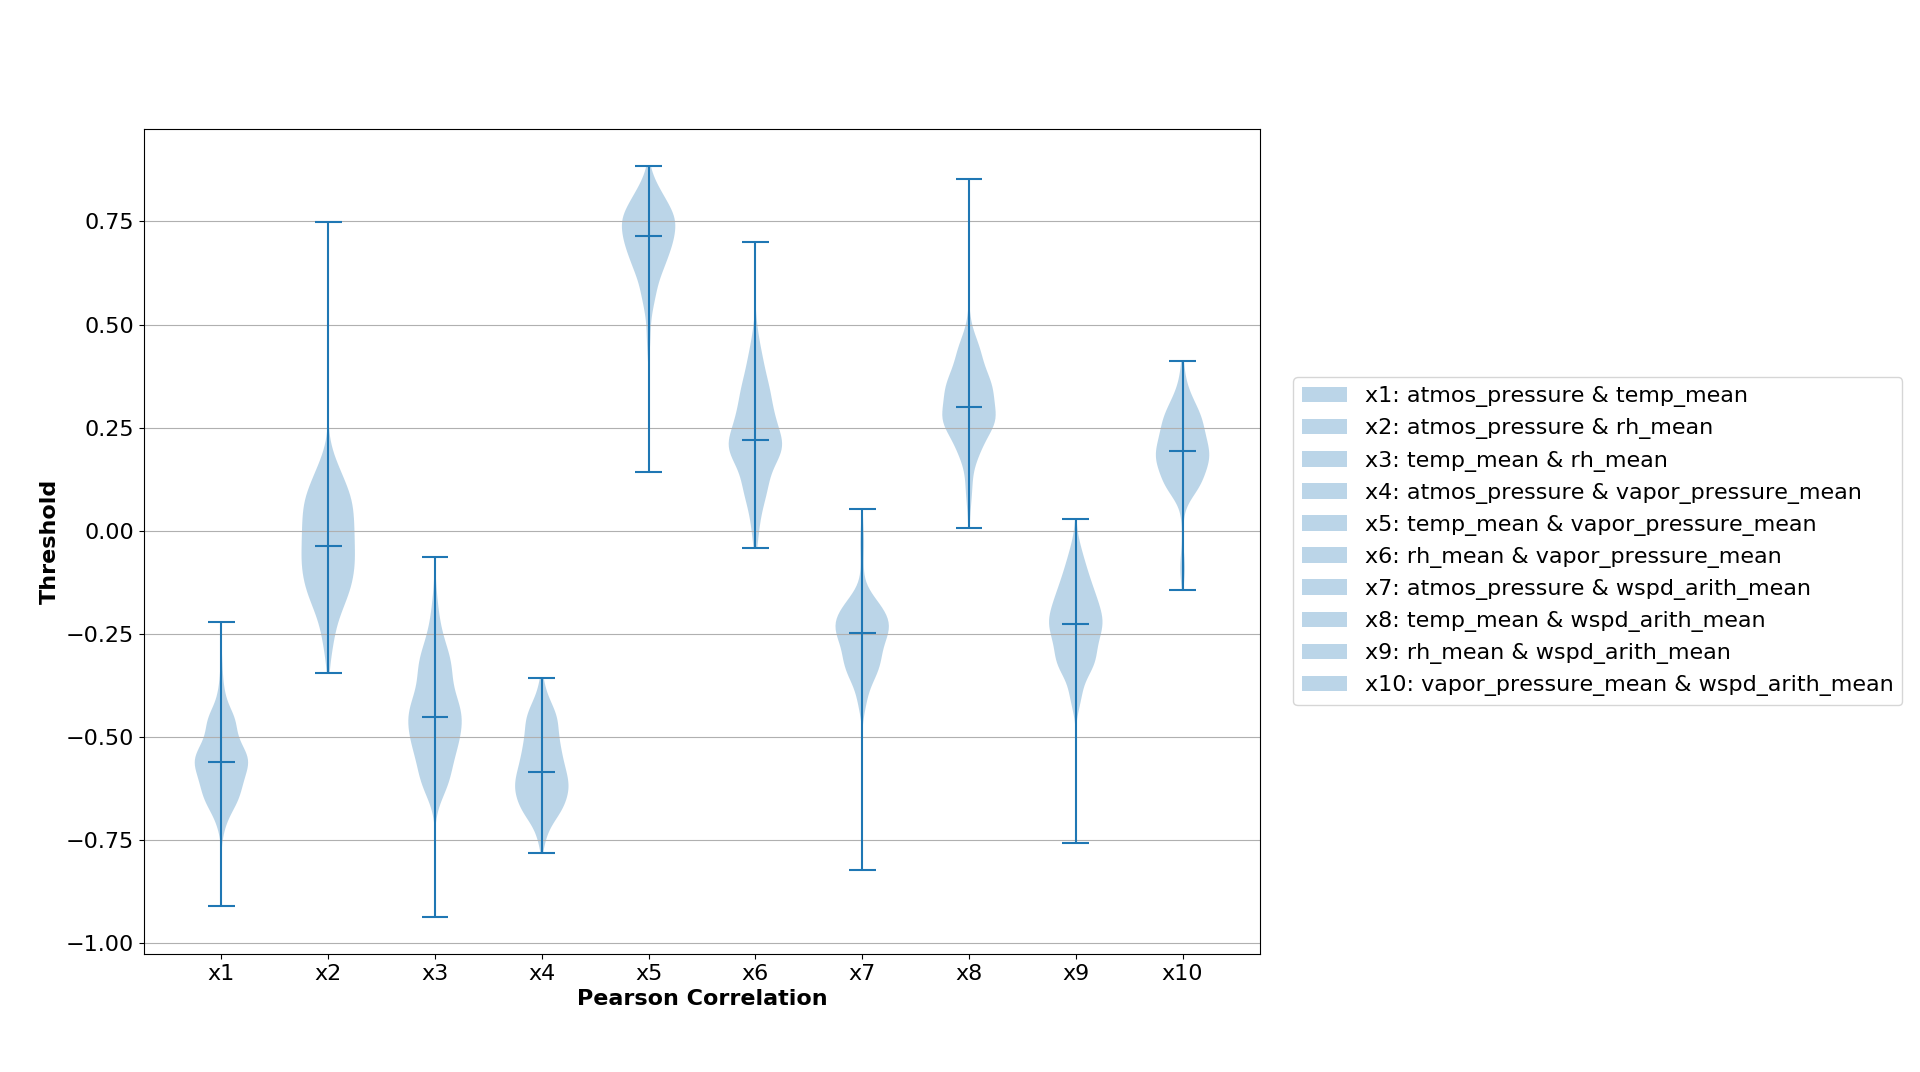
\includegraphics[width=\textwidth]{Spring.png}
    \caption{Violin plot: Spring 5 variables from SGPMET}
    \label{fig:pc}
\end{figure*}

\subsection{Singular Spectrum Analysis}
Singular Spectrum Analysis (SSA) is a popular method for time series data analysis \cite{golyandina2013singular, golyandina2014basic}. The general idea is to use a subset of the decomposition of trajectory matrix to approximate it. Many applications can be found in \cite{golyandina2013singular}. For example, SSA can be applied to monitor volcanic activity \cite{bozzo2010relationship}. It can also be used to extract trend \cite{alexandrov2008method}. Different from the classic SSA method, we defined our own version of SSA to best work on ARM data. Figure 2 is a demonstration of the workflow of SSA. Below is the formal description of the algorithm.

% add workflow of ssa here
\begin{figure}[ht]
    \centering
    % Define block styles
    \tikzstyle{decision} = [diamond, draw, fill=blue!20, text width=4.5em,text badly centered, node distance=3cm, inner sep=0pt]
    \tikzstyle{block} = [rectangle, draw, fill=blue!20, minimum width=5em, text centered, rounded corners, minimum height=2em]
    \tikzstyle{line} = [draw, -latex']
    \tikzstyle{cloud} = [draw, ellipse,fill=red!20, node distance=3cm, text width=3em, minimum height=2em]
    \begin{tikzpicture}[node distance = 2cm, auto]
        % Place nodes
        \node [block] (init) {\small Embedding};
        \node [block, right of=init, node distance=3cm] (decomp) {\small Decomposition};
        \node [block, below of=decomp] (freq) {\small Finding Dominant Frequency};
        \node [block, below of=freq] (period) {\small Converting Periodicity into Frequency};
        \node [block, below of=period] (approx) {\small Approximation};
        \node [block, left of=approx, node distance=3cm] (re) {\small Reconstruction};
        % Draw edges
        \path [line] (init) -- (decomp);
        \path [line] (decomp) -- (freq);
        \path [line] (freq) -- (period);
        \path [line] (period) -- (approx);
        \path [line] (approx) -- (re);
    \end{tikzpicture}
    \caption{Flowchart of SSA}
    \label{fig:pcs}
\end{figure}

% SSA algorithm description
% T = Y.size
% assert L <= T/2
% K = T - L + 1
Assuming we have an ARM data X which has length T.

1) Form the trajectory matrix

2) Find the eigen decomp. 

2) Find the dominant frequency of each eigenvector

3) Convert periodicity into frequency

4) Build an approximation of X by taking a subset of the decomposition. This approximation is formed by taking eigenvectors whose dominant frequency is close to the targeted values.

5) Now we reconstruct the signal by taking a mean of all the approximations.

% The theory behind this method? Need Nate's help
% Input matrix is Y
% trajectory matrix is X

\begin{align*}
X_i = (y_i,\ \ldots,\ y_{i+L-1})^T \quad (1 \leq i \leq K) \\
\mathbf{X} = [X_i,\ \ldots,\ X_K] 
\end{align*}

\begin{equation}
\mathbf{X} = (x_{ij})_{i,j=1}^{L,K}  = \left(\begin{IEEEeqnarraybox*}[][c]{,c/c/c/c/c,}
y_1 & y_2 & y_3 & \ldots & y_K\\
y_2 & y_3 & y_4 & \ldots & y_{K+1}\\
y_3 & y_4 & y_5 & \ldots & y_{K+2}\\
\vdots & \vdots & \vdots & \ddots & \vdots\\
y_L & y_{L+1} & y_{L+2} & \ldots & y_T
\end{IEEEeqnarraybox*}\right)
\end{equation}

\begin{equation}
\mathbf{X} = \mathbf{X_1} + \ldots + \mathbf{X_d}
\end{equation}
where $\mathbf{X_i} = \sqrt{\lambda_i} U_i V_i^T$

\begin{figure*}[ht]
    \centering
    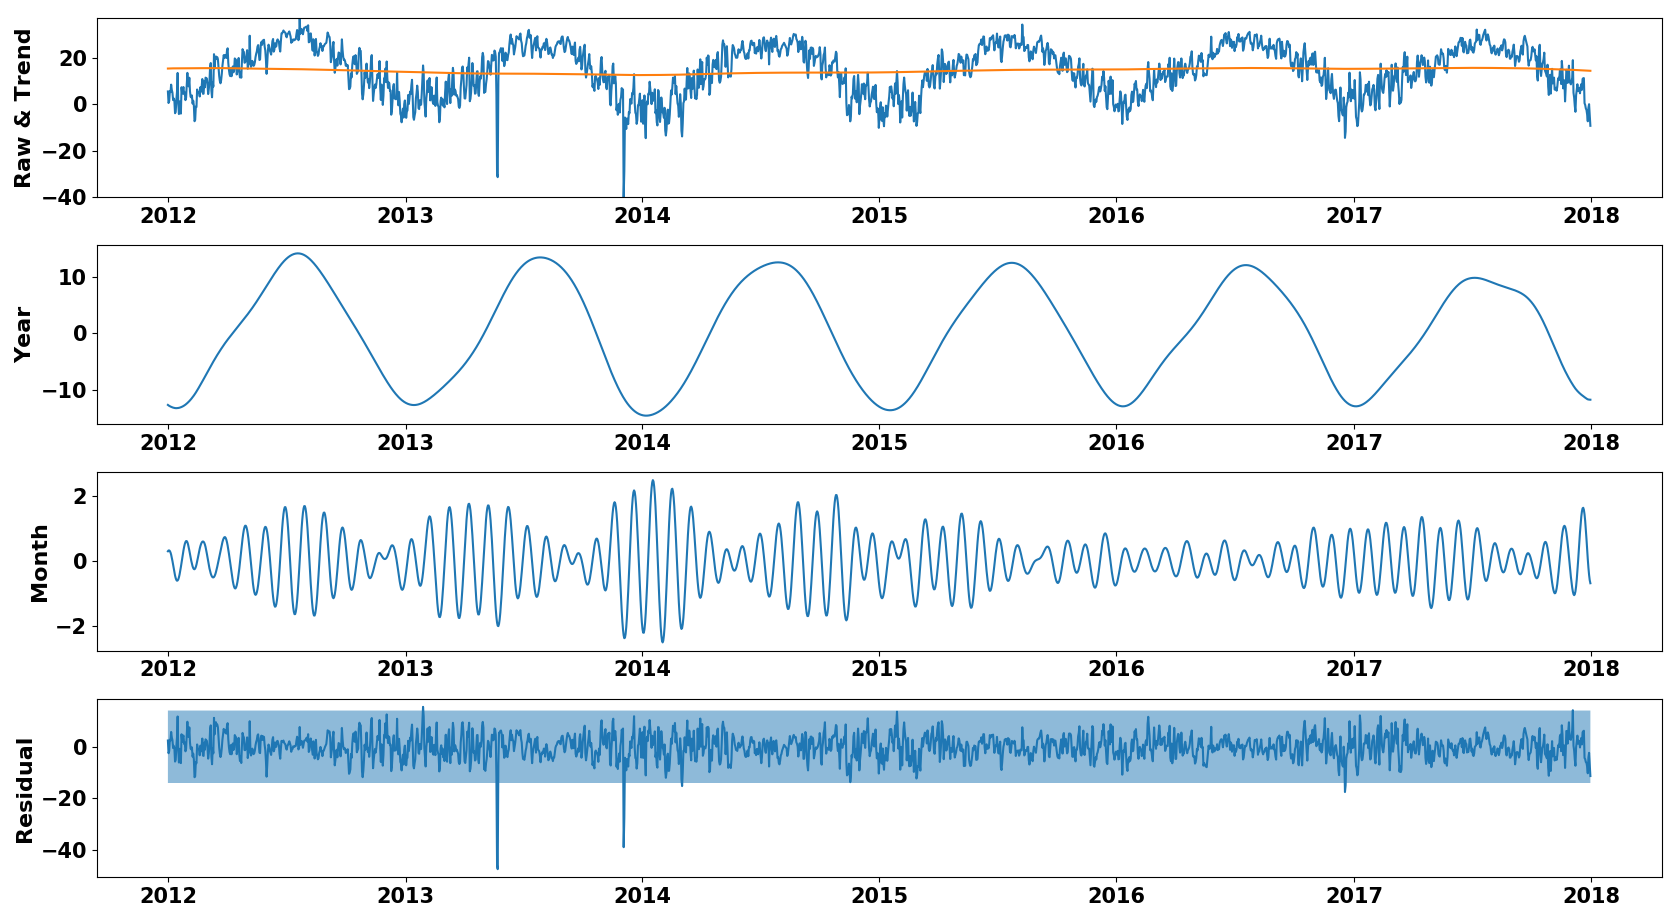
\includegraphics[width=\textwidth]{E33.png}
    \caption{Example of SSA application on ARM data. E33 temp\_mean data full 
    decomposition.}
    \label{fig:ssa}
\end{figure*}

Mention the trend is flat. What parameters do we pick for SSA.


\subsection{K-means}
k-means is a partitioning clustering algorithm \cite{macqueen1967some, hartigan1979algorithm}. It starts with the k centroids user specified, and assigns the points to the nearest centroid. Then it computes the new k centroids and assign other points to these centroids again. The process repeats until it converges.

\begin{figure*}[ht]
    \centering
    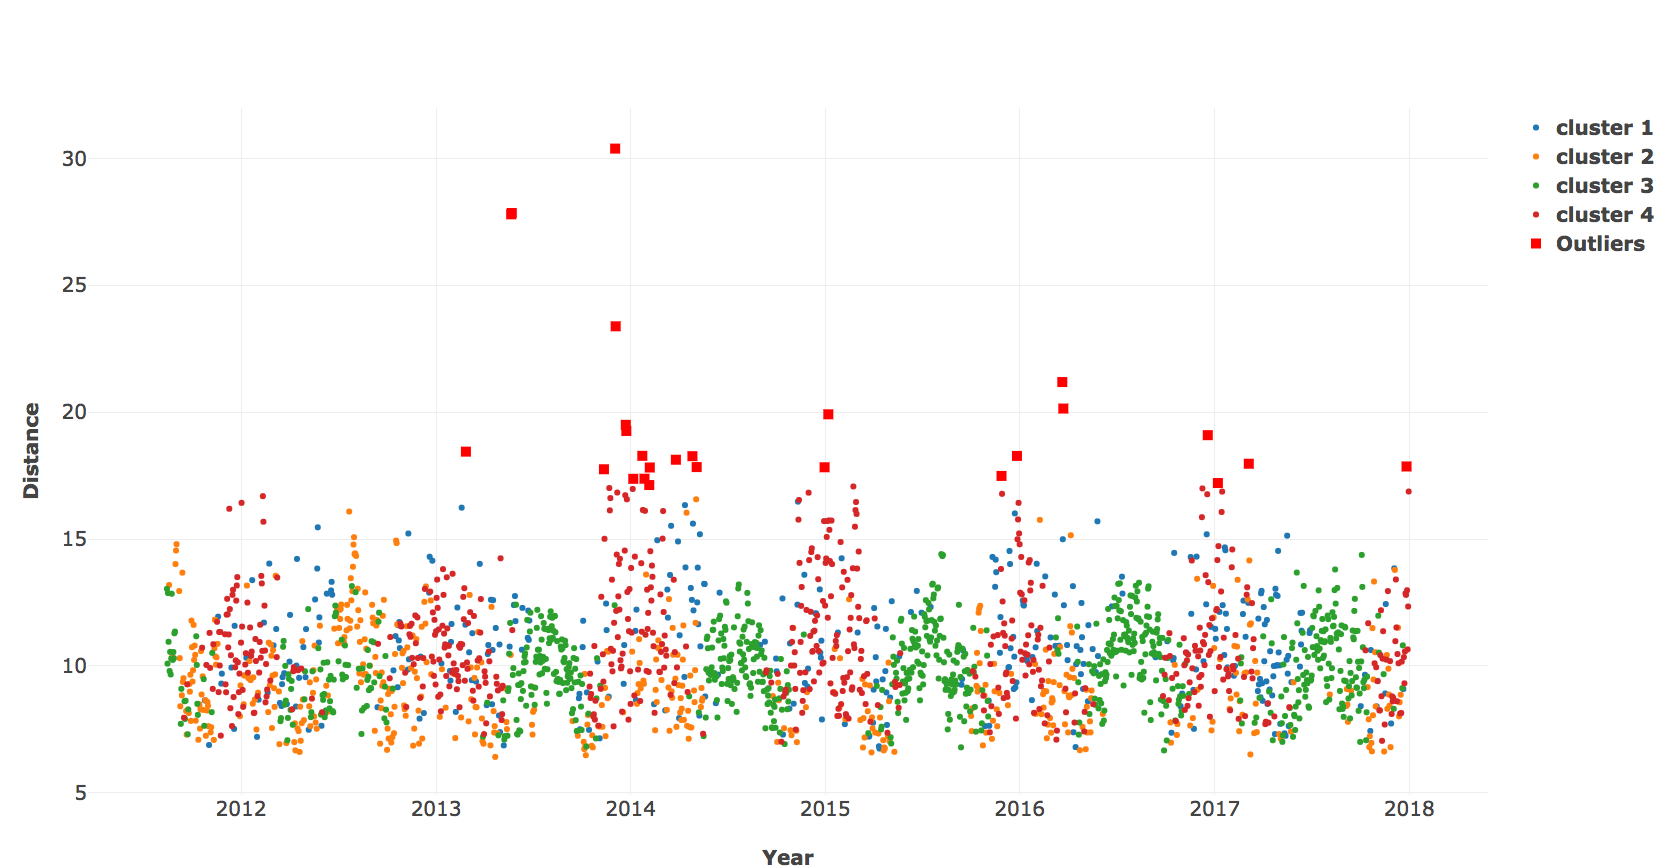
\includegraphics[width=\textwidth]{kmeans.png}
    \caption{E33 K-means}
    \label{fig:kmeans}
\end{figure*}

\section{Results and Discussion}
SSA is an univariate method. K-means is a multivariate method. Results and pics go here. Comparison metric: DQR database. 

Precision and recall was first defined in \cite{perry1955machine}. It is commonly used to measure the quality of classification tasks \cite{olson2008advanced}. Precision is calculated from True Positives divided by the sum of True Positives and False Positives. On the other hand, recall is measured from True Positives divided by the sum of True Positives and False Negatives. In this paper, detected outliers in the DQR database are the ground truth. So we treated these as True Positives. Thus detected outliers not in the DQR database are False Positives. Undetected values which in the DQR database are False Negatives, and which not in the DQR database are True Negatives. Analysis of table 2 and 3 goes here.

\begin{figure*}[ht]
    \centering
    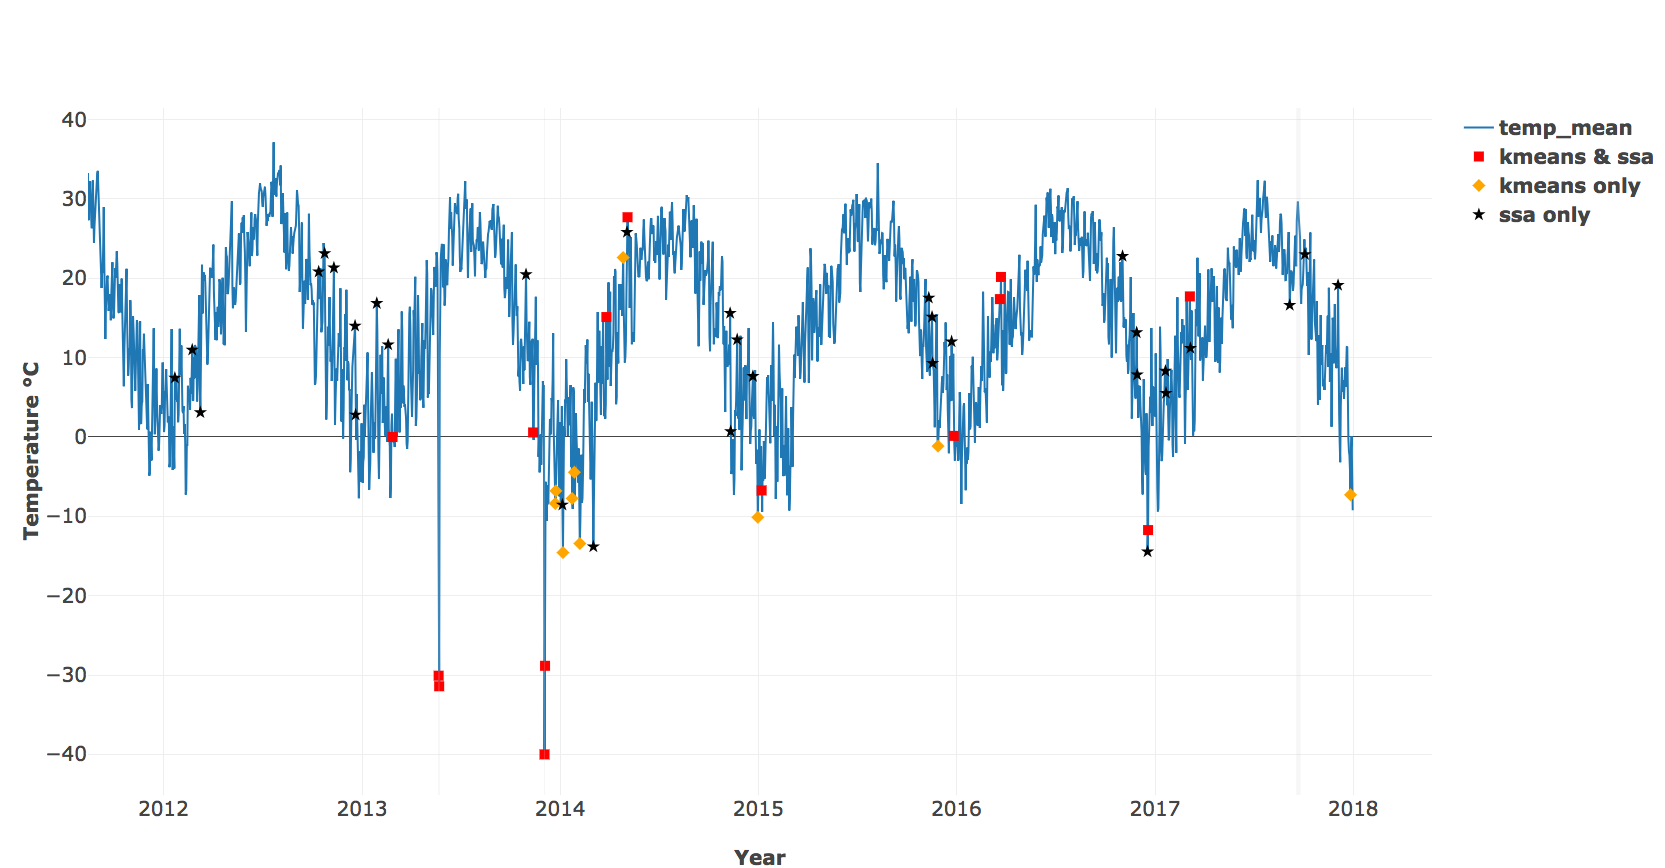
\includegraphics[width=\textwidth]{combined.png}
    \caption{E33 temp\_mean combined}
    \label{fig:combined}
\end{figure*}

\begin{table}[ht]
\caption{Precision and Recall of SSA and K-means}
\label{tab:pr}
\centering
\begin{tabular}{|l|c|c|c|}
\hline
Method & Variable & Precision & Recall\\
\hline
SSA & temp\_mean & 16.00\% & 1.20\%\\
SSA & vapor\_pressure\_mean & 20.70\% & 1.40\%\\
SSA & atmos\_pressure & 0.00\% & 0.00\%\\
SSA & rh\_mean & 14.80\% & 0.50\%\\
SSA & wspd\_arith\_mean & 0.60\% & 1.50\%\\
Kmeans & 5 together & 12.90\% & 1.90\%\\
Combined & 5 together & 11.10\% & 4.10\%\\
\hline
\end{tabular}
\end{table}

\begin{table}[ht]
\caption{Comparison of SSA and K-means Outlier Set Size}
\label{tab:comp}
\centering
\begin{tabular}{|l|c|}
\cline{2-2}
\multicolumn{1}{l|}{} & Outlier Set Size\\
\hline
SSA & 922\\
K-means & 508\\
Intersection & 378\\
Symmetric Difference & 674\\
\hline
\end{tabular}
\end{table}

\section{Conclusions}
We presented a combined model to detect outliers for ARM data. Future work: 
ML and tried methods working on multiple instruments multiple sites \cite{phillips2015graph}.

%\addtolength{\textheight}{-12cm}  % This command serves to balance the column lengths
                                  % on the last page of the document manually. It shortens
                                  % the textheight of the last page by a suitable amount.
                                  % This command does not take effect until the next page
                                  % so it should come on the page before the last. Make
                                  % sure that you do not shorten the textheight too much.

%%%%%%%%%%%%%%%%%%%%%%%%%%%%%%%%%%%%%%%%%%%%%%%%%%%%%%%%%%%%%%%%%%%%%%%%%%%%%%%%
\section*{Acknowledgment}
This research was supported by the Atmospheric Radiation Measurement (ARM) user 
facility, a U.S. Department of Energy (DOE) Office of Science user facility 
managed by the Office of Biological and Environmental Research.


\bibliography{main} 
\bibliographystyle{IEEEtran}


\end{document}